\chapter{Penalty and Augmented Lagrangian Methods}
\label{chap:penalty-augmented-lagrangian}

\section{The Quadratic Penalty Method}

\subsection{Motivation}

\textbf{Idea:} Replace constraints by \textbf{non-negative penalties} that are added to the objective function.

Consider the general problem:
\begin{equation}
    \min_{x \in \mathbb{R}^n} f(x) \quad \text{subject to} \quad
    \begin{cases}
        c_i(x) = 0, & i \in \mathcal{E} \\
        c_i(x) \ge 0, & i \in \mathcal{I}
    \end{cases}
\end{equation}

Define the \textbf{quadratic penalty function} as:
\begin{equation}
    Q(x; \mu) = f(x) + \frac{\mu}{2} \sum_{i \in \mathcal{E}} c_i(x)^2 + \frac{\mu}{2} \sum_{i \in \mathcal{I}} \left[ c_i(x)^- \right]^2
\end{equation}
where $x^- = \max(-x, 0)$ and $\mu > 0$ is the \textbf{penalty parameter}.

The idea is to replace the constrained problem with an \textbf{unconstrained} problem:
\begin{equation}
    \min_{x \in \mathbb{R}^n} Q(x; \mu)
\end{equation}
The objective function of this subproblem contains:
\begin{itemize}
    \item the original objective function $f(x)$;
    \item an additional term for each constraint, which is positive if the constraint is violated, and zero otherwise.
\end{itemize}

\begin{remarque}
    Because of the inequality constraints, the new problem is \textbf{less smooth} due to the max function.
\end{remarque}

\begin{figure}[H]
\centering
\begin{tikzpicture}[scale=1.5]
    \draw[->] (-2.5,0) -- (1.5,0) node[right] {$x$};
    \draw[->] (0,-0.5) -- (0,2.5);
    
    \draw[thick, red] (-2, 2) -- (0, 0) -- (1, 0);
    \node[red, above left] at (-1.8, 2.0) {$x \mapsto x^-$};
    
    \draw[thick, teal, domain=-1.5:0] plot (\x, {\x*\x});
    \draw[thick, teal] (0, 0) -- (1, 0);
    \node[teal, below left] at (-1.4, 2.0) {$x \mapsto (x^-)^2$};
    
    % Dashed lines for x=-1
    \draw[dashed, gray] (-1, 0) node[below] {$-1$} -- (-1, 1);
    \draw[dashed, gray] (-1, 1) -- (0, 1) node[right] {$1$};
    
    % Origin
    \node[below right] at (0,0) {$0$};
    
\end{tikzpicture}
\caption{Comparison of penalty functions for an inequality $x \ge 0$. In red, the exact penalty $x^-$ (non-differentiable at 0). In green, the quadratic penalty $(x^-)^2$ (differentiable, $C^1$).}
\label{fig:penalty-functions-comparison}
\end{figure}

\begin{figureexplanation}
The linear penalty $x^-$ has a kink at the origin (non-differentiable), while $(x^-)^2$ is smooth and tangent to the axis. This differentiability allows the application of gradient methods.
\end{figureexplanation}

\paragraph{Example:}
Let $\min_{x \in \mathbb{R}^2} x_1 + x_2$ subject to $x_1^2 + x_2^2 - 2 = 0$.
The quadratic penalty function is:
\begin{equation}
    Q(x; \mu) = x_1 + x_2 + \frac{\mu}{2} (x_1^2 + x_2^2 - 2)^2
\end{equation}
The gradient vanishes when (with $x_1 = x_2$ by symmetry):
\begin{equation}
    1 + 4\mu x_1 (x_1^2 - 1) = 0
\end{equation}
There exists a local minimum that tends to $(-1, -1)$ as $\mu \to \infty$.

\begin{figure}[H]
\centering
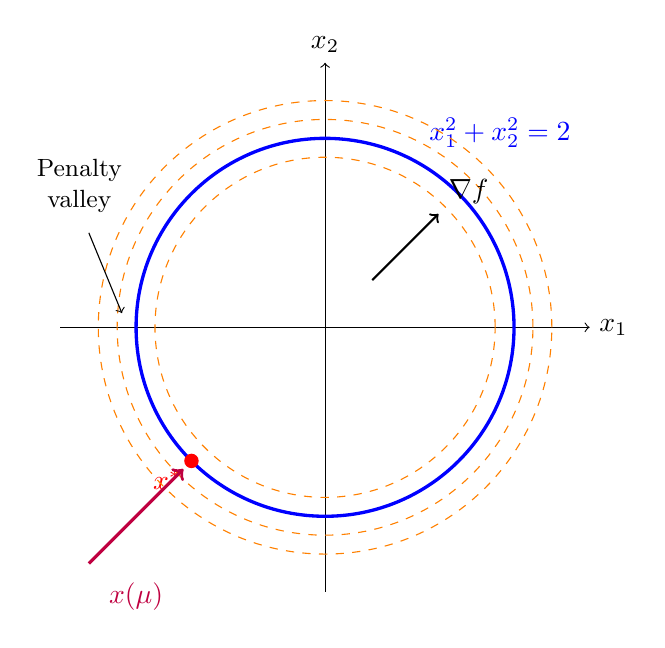
\begin{tikzpicture}[scale=1.2]
    \draw[->] (-2.8,0) -- (2.8,0) node[right] {$x_1$};
    \draw[->] (0,-2.8) -- (0,2.8) node[above] {$x_2$};
    
    \draw[very thick, blue] (0,0) circle (2);
    \node[blue, above right] at (1.0, 1.8) {$x_1^2+x_2^2=2$};
    \filldraw[red] (-1.414, -1.414) circle (2pt) node[below left] {$x^*$};
    
    % Penalty Contours
    \draw[orange, thin, dashed] (0,0) circle (2.2);
    \draw[orange, thin, dashed] (0,0) circle (1.8);
    \draw[orange, thin, dashed] (0,0) circle (2.4);
    
    \draw[->, black, thick] (0.5, 0.5) -- (1.2, 1.2) node[above right] {$\nabla f$};
    
    \draw[->, purple, very thick] (-2.5, -2.5) -- (-1.5, -1.5);
    \node[purple, below] at (-2.0, -2.6) {$x(\mu)$};
    
    \node[align=center, font=\small] at (-2.6, 1.5) {Penalty\\valley};
    \draw[->] (-2.5, 1.0) -- (-2.15, 0.15);
    
\end{tikzpicture}
\caption{Penalty method: As $\mu$ increases, the function $Q(x;\mu)$ forms a steep "valley" along the constraint $c(x)=0$. The sequence of minimizers $x(\mu)$ (purple arrow) descends to the bottom of this valley while approaching the constraint, finally ending at $x^*$.}
\label{fig:penalty-valley}
\end{figure}

\begin{figureexplanation}
\textbf{The penalty "valley":}
Imagine the constraint (the blue circle) is the bottom of a canyon.
\begin{itemize}
    \item Far from the circle, the penalty term $\frac{\mu}{2} c(x)^2$ is huge: the walls of the canyon are very high.
    \item To minimize $Q$, one must descend to the bottom of the canyon ($c(x) \approx 0$).
    \item Once at the bottom, we try to minimize the original function $f(x)$ by moving \emph{along} the constraint.
    \item Numerical problem: The bottom is somewhat "flat" in the constraint direction, but the walls are very steep. This creates an ill-conditioned ("long and narrow") Hessian matrix.
\end{itemize}
\end{figureexplanation}

\begin{algorithm}[H]
    \caption{Quadratic Penalty Method}
    \SetAlgoLined
    Given: $\mu_0 > 0$, a nonnegative sequence $\{\tau_k\}$ with $\tau_k \to 0$, and a starting point $x_0^s$\;
    \For{$k=0, 1, \ldots$}{
        Find an approximate minimizer $x_k$ of $Q(\cdot;\mu_k)$, starting at $x_k^s$, and terminating when $\|\nabla_x Q(x;\mu_k)\|\leq \tau_k$\;
        \If{final convergence test satisfied}{
            \Stop with approximate solution $x_k$\;
        }
        Choose new penalty parameter $\mu_{k+1} > \mu_k$\;
        Choose new starting point $x_{k+1}^s$\;
    }
\end{algorithm}

\subsection{Convergence of the Method (with Equality Constraints)}

\begin{theoreme}[Global Convergence]
    Suppose that each $x_k$ is the exact minimizer of $Q(\cdot; \mu_k)$ and that $\mu_k \uparrow \infty$.
    Then, any limit point $x^*$ of the sequence $\{x_k\}$ is a global solution to the problem.
\end{theoreme}

\begin{proof}
    Let $\bar{x}$ be a global solution to the constrained problem.
    Then $\bar{x}$ is feasible, i.e., $c_i(\bar{x}) = 0$ for all $i \in \mathcal{E}$.
    By definition of $x_k$ as the minimizer of $Q(\cdot; \mu_k)$, we have:
    \[
        Q(x_k; \mu_k) \le Q(\bar{x}; \mu_k).
    \]
    Expanding the expression of the penalty function:
    \[
        f(x_k) + \frac{\mu_k}{2} \sum_{i \in \mathcal{E}} c_i(x_k)^2 \le f(\bar{x}) + \frac{\mu_k}{2} \sum_{i \in \mathcal{E}} c_i(\bar{x})^2.
    \]
    Since $\bar{x}$ is feasible, the penalty term for $\bar{x}$ is zero:
    \[
        f(x_k) + \frac{\mu_k}{2} \sum_{i \in \mathcal{E}} c_i(x_k)^2 \le f(\bar{x}).
    \]
    Rearranging this inequality to isolate the constraint violation term:
    \[
        \sum_{i \in \mathcal{E}} c_i(x_k)^2 \le \frac{2}{\mu_k} [f(\bar{x}) - f(x_k)].
    \]
    Suppose $x^*$ is a limit point of the sequence $\{x_k\}$. There exists a subsequence $\mathcal{K}$ such that:
    \[
        \lim_{k \in \mathcal{K}} x_k = x^*.
    \]
    Take the limit in the previous inequality for $k \in \mathcal{K}$ tending to infinity. Since $\mu_k \to \infty$, the right-hand side tends to 0 (assuming $f(x_k)$ is bounded or converges to $f(x^*)$):
    \[
        \sum_{i \in \mathcal{E}} c_i(x^*)^2 = \lim_{k \in \mathcal{K}} \sum_{i \in \mathcal{E}} c_i(x_k)^2 \le 0.
    \]
    Since a sum of squares is always non-negative, we deduce that $\sum c_i(x^*)^2 = 0$, and thus:
    \[
        c_i(x^*) = 0, \quad \forall i \in \mathcal{E}.
    \]
    Therefore, $x^*$ is a feasible point.
    
    Moreover, returning to the inequality $f(x_k) + \text{penalty} \le f(\bar{x})$. Since the penalty term is non-negative, we have simply:
    \[
        f(x_k) \le f(\bar{x}).
    \]
    Passing to the limit over the subsequence $\mathcal{K}$:
    \[
        f(x^*) \le f(\bar{x}).
    \]
    Since $x^*$ is feasible and its objective value is less than or equal to that of the global solution $\bar{x}$, $x^*$ is itself a global solution.
\end{proof}

\begin{remarque}
    In practice, finding the exact minimizer is not realistic at every step.
\end{remarque}

\begin{theoreme}[KKT Convergence]
    Suppose that the tolerances and penalties satisfy $\tau_k \downarrow 0$ and $\mu_k \uparrow \infty$.
    Then, if a limit point $x^*$ of the sequence $\{x_k\}$ is \textbf{infeasible}, then $x^*$ is a stationary point of the function $x \mapsto \|c(x)\|^2 = \sum_{i \in \mathcal{E}} [c_i(x)]^2$.
    
    On the other hand, if $x^*$ is \textbf{feasible} and if the constraint gradients $\nabla c_i(x^*)$ are linearly independent (LICQ), then $x^*$ is a KKT point for the problem.
\end{theoreme}

\begin{remarque}[Lagrange Multipliers]
    For such points, for any index subsequence $\mathcal{K}$ such that $x^* = \lim_{k \in \mathcal{K}} x_k$, we have:
    \[
        \lim_{k \in \mathcal{K}} (-\mu_k c_i(x_k)) = \lambda_i^*, \quad \text{for all } i \in \mathcal{E},
    \]
    where $\lambda^*$ are the Lagrange multipliers associated with $x^*$ for the original problem.
    \begin{proof}
        See Nocedal and Wright.
    \end{proof}
\end{remarque}

\begin{remarque}[Ill-conditioning of the Hessian]
    The Hessian of the penalty function is given by:
    \[
        \nabla_{xx}^2 Q(x; \mu_k) = \nabla^2 f(x) + \sum_{i \in \mathcal{E}} \mu_k c_i(x) \nabla^2 c_i(x) + \mu_k A(x)^\top A(x),
    \]
    where $A(x)^\top = [\nabla c_i(x)]_{i \in \mathcal{E}}$.
    
    When $x$ is close to the minimizer of $Q(\cdot; \mu_k)$, the conditions of the theorem are satisfied and we have the approximation:
    \[
        \nabla_{xx}^2 Q(x; \mu_k) \approx \nabla_{xx}^2 \mathcal{L}(x, \lambda^*) + \mu_k A(x)^\top A(x).
    \]
    The matrix $\nabla_{xx}^2 \mathcal{L}(x, \lambda^*)$ is independent of $\mu_k$.
    The term $\mu_k A(x)^\top A(x)$ has rank $|\mathcal{E}|$ (since $A(x)$ has $|\mathcal{E}|$ rows which are the assumed independent gradients).
    
    Thus, the Hessian has $|\mathcal{E}|$ eigenvalues of order $\mu_k$ (from $A^\top A$) and $n - |\mathcal{E}|$ eigenvalues of order 1 (from the Lagrangian).
    This matrix is singular when $|\mathcal{E}| < n$ for the dominant term.
    
    Since $\mu_k \to \infty$, the condition number of the matrix explodes: $\nabla_{xx}^2 Q(\cdot; \mu_k)$ becomes ill-conditioned. This makes minimization by Newton or quasi-Newton methods difficult.
\end{remarque}

\paragraph{Consequence on the computation of the Newton step:}
    We seek to solve $\nabla_{xx}^2 Q(x; \mu_k) p_N = -\nabla_x Q(x; \mu_k)$.
    To avoid numerical errors due to ill-conditioning, an auxiliary variable $\zeta = \mu_k A(x) p_N$ is introduced.
    The system can then be rewritten in the form:
    \[
    \begin{pmatrix}
        \nabla^2 f(x) + \sum_{i \in \mathcal{E}} \mu_k c_i(x) \nabla^2 c_i(x) & A(x)^\top \\
        A(x) & -\frac{1}{\mu_k} I
    \end{pmatrix}
    \begin{pmatrix}
        p_N \\
        \zeta
    \end{pmatrix}
    =
    \begin{pmatrix}
        -\nabla_x Q(x; \mu_k) \\
        0
    \end{pmatrix}
    \]
    This formulation avoids explicitly forming the ill-conditioned matrix $\mu_k A^\top A$.

\section{Nonsmooth Penalty Functions ($l^1$)}

\subsection{Definition and Properties}

A popular alternative is the $l^1$ penalty function, defined by:
\[
    \phi_1(x; \mu) = f(x) + \mu \sum_{i \in \mathcal{E}} |c_i(x)| + \mu \sum_{i \in \mathcal{I}} [c_i(x)]^-,
\]
where $[y]^- = \max(-y, 0)$.

Unlike the quadratic penalty, this function is not differentiable at points where $c_i(x) = 0$. However, it has a very important property: it is an \textbf{exact penalty function}.

\begin{theoreme}[Exact Penalty]
    Suppose that $x^*$ is a strict local solution of the constrained problem:
    \[
        \min f(x) \quad \text{s.t. } \quad c_i(x) = 0, \; i \in \mathcal{E}, \quad c_i(x) \ge 0, \; i \in \mathcal{I},
    \]
    and that the first-order KKT conditions are satisfied for some multipliers $\lambda^*$.
    
    Then, $x^*$ is a local minimum of $\phi_1(\cdot; \mu)$ for all $\mu > \mu^*$, where
    \[
        \mu^* = \|\lambda^*\|_\infty = \max_i |\lambda_i^*|.
    \]
    If the second-order sufficient conditions are also satisfied, then $x^*$ is a \textbf{strict} local minimum.
\end{theoreme}

\begin{figure}[H]
    \centering
    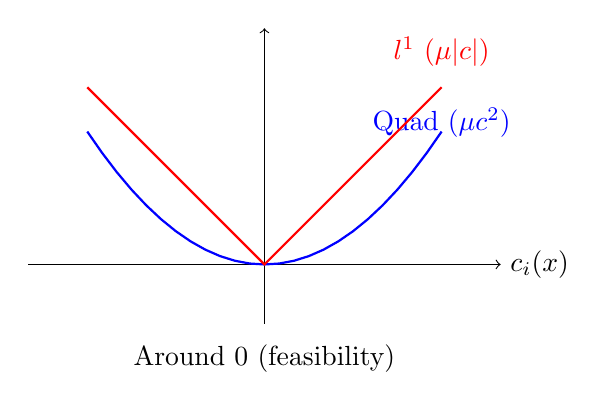
\begin{tikzpicture}[scale=1.5]
        \draw[->] (-2,0) -- (2,0) node[right] {$c_i(x)$};
        \draw[->] (0,-0.5) -- (0,2);
        
        \draw[blue, thick, domain=-1.5:1.5] plot (\x, {0.5*\x*\x});
        \node[blue] at (1.5, 1.2) {Quad ($\mu c^2$)};
        
        % L1
        \draw[red, thick] (-1.5, 1.5) -- (0,0) -- (1.5, 1.5);
        \node[red] at (1.5, 1.8) {$l^1$ ($\mu |c|$)};
        
        \node[align=center] at (0, -0.8) {Around $0$ (feasibility)};
    \end{tikzpicture}
    \caption{Comparison: The quadratic penalty (blue) is smooth but has zero slope at the origin, requiring $\mu \to \infty$ to force $c(x) \to 0$. The $l^1$ penalty (red) has a non-zero slope ("kink") at the origin, allowing an exact solution for finite $\mu$.}
\end{figure}

\subsection{Characterization of Behavior}

We wish to study the stationary points of $\phi_1$, which is not differentiable.
For this, we use directional derivatives.

\begin{definition}[Directional derivative]
    The directional derivative of $f: \mathbb{R}^n \to \mathbb{R}$ in the direction $p \in \mathbb{R}^n$ is given by:
    \[
        D(f(x), p) = \lim_{\epsilon \to 0} \frac{f(x + \epsilon p) - f(x)}{\epsilon}.
    \]
\end{definition}

\begin{definition}[Stationarity]
    A point $\hat{x} \in \mathbb{R}^n$ is a stationary point for the penalty function $\phi_1(\cdot; \mu)$ if:
    \[
        D(\phi_1(\hat{x}; \mu), p) \ge 0, \quad \text{for all } p \in \mathbb{R}^n.
    \]
\end{definition}

We also define an infeasibility measure:
\[
    h(x) = \sum_{i \in \mathcal{E}} |c_i(x)| + \sum_{i \in \mathcal{I}} [c_i(x)]^-.
\]
A point $\hat{x}$ is a "stationary point for the infeasibility measure" if $D(h(\hat{x}); p) \ge 0$ for all $p \in \mathbb{R}^n$.
If in addition $x$ is infeasible for the original problem, we call it an \textbf{infeasible stationary point}.

\begin{theoreme}
    Suppose that $\hat{x}$ is a stationary point for the penalty function $\phi_1(\cdot; \mu)$ for all $\mu > \mu^*$.
    Then:
    \begin{itemize}
        \item If $\hat{x}$ is feasible for the problem, then it satisfies the KKT conditions.
        \item Otherwise, it is an infeasible stationary point.
    \end{itemize}
\end{theoreme}

\begin{exemple}
    Consider the problem:
    \[
        \min_{x \in \mathbb{R}^2} x_1 + x_2 \quad \text{s.t.} \quad x_1^2 + x_2^2 - 2 = 0.
    \]
    The $l^1$ penalty function is:
    \[
        \phi_1(x; \mu) = x_1 + x_2 + \mu |x_1^2 + x_2^2 - 2|.
    \]
    It can be shown that the minimizer of $\phi_1(\cdot; \mu)$ is the solution $(-1, -1)$ for all $\mu > \mu^* = 0.5$.
\end{exemple}

\section{Practical Approach: Modified $l^1$ Model}

Since $\phi_1(\cdot; \mu)$ is nonsmooth, one cannot directly apply Newton's method.
A practical approach (Framework 20) consists of forming a modified model by:
\begin{itemize}
    \item Linearizing the constraints $c_i$.
    \item Replacing $f$ by a quadratic approximation.
\end{itemize}
We then seek to minimize with respect to $p$ the function:
\[
    q(p; \mu) = f(x) + \nabla f(x)^\top p + \frac{1}{2} p^\top W p + \mu \sum_{i \in \mathcal{E}} |c_i(x) + \nabla c_i(x)^\top p| + \mu \sum_{i \in \mathcal{I}} [c_i(x) + \nabla c_i(x)^\top p]^-,
\]
where $W$ is an approximation of the Hessian of the Lagrangian.
This model $q(p; \mu)$ is nonsmooth. However, if $W$ is positive definite, this subproblem can be reformulated as a smooth quadratic program (QP) by introducing artificial variables $r, s, t$:
\[
    \min_{p, r, s, t} \nabla f(x)^\top p + \frac{1}{2} p^\top W p + \mu \sum_{i \in \mathcal{E}} (r_i + s_i) + \mu \sum_{i \in \mathcal{I}} t_i
\]
subject to the constraints:
\[
    \begin{cases}
        \nabla c_i(x)^\top p + c_i(x) = r_i - s_i, & i \in \mathcal{E} \\
        \nabla c_i(x)^\top p + c_i(x) \ge -t_i, & i \in \mathcal{I} \\
        r, s, t \ge 0
    \end{cases}
\]
This problem can be efficiently solved by standard QP solvers.

\section{Augmented Lagrangian Methods}

\subsection{Definition and Motivation}

We have seen that for the quadratic penalty, the sequence $\{x_k\}$ converges to a solution, but it requires that $\mu_k \to \infty$. This leads to ill-conditioning of the Hessian.
Moreover, we have the asymptotic relationship:
\[
    \lim_{k \to \infty} -\mu_k c_i(x_k) = \lambda_i^*.
\]
The idea of Augmented Lagrangian methods is to use an explicit estimate of the Lagrange multipliers $\lambda$ to avoid having to send $\mu$ to infinity too quickly.

We define the \textbf{Augmented Lagrangian} $\mathcal{L}_A$ by:
\[
    \mathcal{L}_A(x, \lambda; \mu) = f(x) - \sum_{i \in \mathcal{E}} \lambda_i c_i(x) + \frac{\mu}{2} \sum_{i \in \mathcal{E}} c_i(x)^2.
\]
This function combines the Lagrangian and the quadratic penalty.

\subsection{Algorithm (Method of Multipliers)}

The proposed algorithm is as follows:
\begin{enumerate}
    \item At iteration $k$, we fix an estimate of the multipliers $\lambda^k$ and a penalty $\mu_k > 0$.
    \item We seek a minimizer $x_k$ of $\mathcal{L}_A(\cdot, \lambda^k; \mu_k)$. The optimality condition is:
    \[
        \nabla_x \mathcal{L}_A(x_k, \lambda^k; \mu_k) = \nabla f(x_k) - \sum_{i \in \mathcal{E}} (\lambda_i^k - \mu_k c_i(x_k)) \nabla c_i(x_k) \approx 0.
    \]
    \item By comparing with the KKT condition $\nabla f(x^*) - \sum \lambda_i^* \nabla c_i(x^*) = 0$, this suggests the following update rule for the multipliers:
    \[
        \lambda_i^{k+1} = \lambda_i^k - \mu_k c_i(x_k).
    \]
\end{enumerate}

\paragraph{Comparison of behavior:}
\begin{itemize}
    \item \textbf{Before (Quadratic Penalty only):} We had $-\mu_k c_i(x_k) \approx \lambda_i^*$, which implied $c_i(x_k) \approx -\frac{\lambda_i^*}{\mu_k}$. To have $c_i$ small, an extremely large $\mu_k$ was needed.
    \item \textbf{With Augmented Lagrangian:} The condition becomes $\lambda_i^k - \mu_k c_i(x_k) \approx \lambda_i^*$.
    Thus:
    \[
        c_i(x_k) \approx \frac{\lambda_i^k - \lambda_i^*}{\mu_k}.
    \]
    If $\lambda^k$ converges to $\lambda^*$, the numerator tends to 0. We can therefore obtain a small constraint violation $c_i(x_k)$ even without $\mu_k$ going to infinity.
\end{itemize}



\section{Augmented Lagrangian Method}

\subsection{Properties of the equality-constrained case}

\begin{algorithm}[H]
    \caption{Augmented Lagrangian method for equality constraints}
    \SetAlgoLined
    Given $\mu_0>0$, tolerance $\tau_0>0$, starting points $x_0^s$ and $\lambda^0$\;
    \For{$k=0, 1, \ldots$}{
        Find an approximate minimizer $x_k$ of $\mathcal{L}_A(\cdot, \lambda^k;\mu_k)$, starting at $x_k^s$, and terminating when $\|\nabla_x \mathcal{L}_A(x_k, \lambda^k; \mu_k)\| \leq \tau_k$\;
        \If{a convergence test for the equality-constrained problem is satisfied}{
            \Stop with approximate solution $x_k$\;
        }
        Update Lagrange multipliers using
        \[
            \lambda_i^{k+1} = \lambda_i^k - \mu_k c_i(x_k), \text{ for all } i\in\mathcal{E};
        \]
        Choose new penalty parameter $\mu_{k+1} \geq \mu_k$\;
        Set starting point for the next iteration to $x_{k+1}^s = x_k$\;
        Select tolerance $\tau_{k+1}$\;
    }
\end{algorithm}

\subsection{Practical Augmented Lagrangian Methods}

\subsubsection{Formulation with bound constraints}

\begin{algorithm}[H]
    \caption{Bound-constrained Lagrangian method}
    \SetAlgoLined
    Choose an initial point $x_0$ and initial multipliers $\lambda^0$\;
    Choose convergence tolerances $\eta_*$ and $\omega_*$\;
    Set $\mu_0=10$, $\omega_0=\frac{1}{\mu_0}$, and $\eta_0=\frac{1}{\mu_0^{0.1}}$\;
    \For{$k=0,1, \ldots$}{
        Find an approximate solution $x_k$ of the problem
        \[
            \min_x \mathcal{L}_A(x,\lambda^k;\mu_k) \text{ subject to } l\leq x\leq u
        \]
        such that
        \[
            \left\| x_k-P\left(x_k - \nabla_x \mathcal{L}_A(x_k, \lambda^k ; \mu_k), l, u\right) \right\| \leq \omega_k;
        \]
        \If{$\|c(x_k)\|\leq \eta_k$}{
            \Comment{test for convergence}
            \If{$\|c(x_k)\|\leq \eta_*$ \And $\left\| x_k-P\left(x_k - \nabla_x \mathcal{L}_A(x_k, \lambda^k ; \mu_k), l, u\right) \right\| \leq \omega_*$}{
                \Stop with approximate solution $x_k$\;
            }
            \Comment{update multipliers, tighten tolerances}
            $\lambda^{k+1}\leftarrow \lambda^k - \mu_k c(x_k)$\;
            $\mu_{k+1}\leftarrow \mu_k$\;
            $\eta_{k+1}\leftarrow \frac{\eta_k}{\mu_{k+1}^{0.9}}$\;
            $\omega_{k+1} \leftarrow \frac{\omega_k}{\mu_{k+1}}$\;
        }
        \Else{
            \Comment{increase penalty parameters, tighten tolerances}
            $\lambda^{k+1}\leftarrow \lambda^k$\;
            $\mu_{k+1}\leftarrow 100 \mu_k$\;
            $\eta_{k+1}\leftarrow \frac{1}{\mu_{k+1}^{0.1}}$\;
            $\omega_{k+1} \leftarrow \frac{1}{\mu_{k+1}}$\;
        }
    }
\end{algorithm}



%%%%%%%%%%%%%%%%%%%%%%%%%%%%%%%%%%%%%%%%%%%%%%%%%%%%%%%%%%%%
\section{Practice Exercises (Nocedal \& Wright)}
\label{sec:12.exercises}

Exercises related to Chapter 17 of the book (Penalty and Augmented Lagrangian Methods).

\bigskip
\begin{exercice}[Convergence of the quadratic penalty method]
Verify that if $x^*$ is a solution to the constrained problem, then it is a stationary point of the quadratic penalty function $Q(x; \mu)$ as $\mu \to \infty$. 
(See Theorem 17.1 and Exercise 17.1 of the book).
\end{exercice}

\begin{correction}
$\nabla Q(x; \mu) = \nabla f(x) + \mu \sum c_i(x) \nabla c_i(x)$.
For $\nabla Q \to 0$, $\nabla f$ must be balanced by the penalty term.
In the limit, $x_k \to x^*$.
If $x^*$ is feasible, $c_i(x^*) = 0$.
The limit relationship gives $\nabla f(x^*) + \sum \lambda_i^* \nabla c_i(x^*) = 0$ (KKT), where $\lambda_i^* \approx -\mu c_i(x_k)$.
\end{correction}
\bigskip

\bigskip
\begin{exercice}[Comparison of Augmented Lagrangian vs Penalty]
Study Example 17.4 (page 536 of the Nocedal/Wright book) which compares the conditioning of the two methods for the problem:
$$ \min x_1 + x_2 \quad \text{s.t. } x_1^2 + x_2^2 - 2 = 0 $$
Show that the Augmented Lagrangian converges better and with better conditioning than the simple penalty.
\end{exercice}

\begin{correction}
The circle $x_1^2 + x_2^2 = 2$ is the constraint. Solution $x^*=(-1,-1)$.
Simple Penalty: The contours become very elongated ("valley") around the constraint, making minimization difficult (ill-conditioning of the Hessian).
Augmented Lagrangian: The linear term $-\lambda^\top c(x)$ "shifts" the bottom of the valley so that it coincides with the constraint without needing an immense $\mu$.
This allows finding the precise solution with a moderate $\mu$, thus with better conditioning.
\end{correction}
\bigskip

\bigskip
\begin{exercice}[Explicit Computation - Penalty Method]
Consider the scalar problem:
$$ \min_{x \in \mathbb{R}} \frac{1}{2}x^2 \quad \text{s.t. } x = 1 $$
\begin{enumerate}
    \item Write the quadratic penalty function $Q(x; \mu)$.
    \item Find the minimizer $x_\mu$ of $Q(x; \mu)$ for a given $\mu > 0$.
    \item Verify that $x_\mu \to x^*$ (the exact solution) as $\mu \to \infty$.
    \item Estimate the Lagrange multiplier $\lambda^*$ from $x_\mu$ and verify its convergence.
\end{enumerate}
\end{exercice}

\begin{correction}
\textbf{1. Penalty Function:}
$Q(x; \mu) = \frac{1}{2}x^2 + \frac{\mu}{2}(x-1)^2$.

\textbf{2. Minimizer $x_\mu$:}
$Q'(x) = x + \mu(x-1) = 0$.
$x(1+\mu) = \mu \implies x_\mu = \frac{\mu}{1+\mu}$.

\textbf{3. Primal Convergence:}
$\lim_{\mu \to \infty} x_\mu = \lim \frac{\mu}{\mu} = 1$.
The exact solution to the problem is obviously $x^*=1$. Convergence verified.

\textbf{4. Dual Multiplier:}
Exact KKT: $L = \frac{1}{2}x^2 - \lambda(x-1)$. $\nabla L = x - \lambda = 0 \implies \lambda^* = x^* = 1$.
Penalty estimate (Formula $\lambda \approx -\mu c(x)$ for $L = f - \lambda c$):
$\lambda_\mu = -\mu (x_\mu - 1) = -\mu (\frac{\mu}{1+\mu} - 1) = -\mu (\frac{\mu - (1+\mu)}{1+\mu}) = -\mu (\frac{-1}{1+\mu}) = \frac{\mu}{1+\mu}$.
As $\mu \to \infty$, $\lambda_\mu \to 1$.
Convergence verified towards $\lambda^* = 1$.
\end{correction}
\bigskip

\bigskip
\begin{checkpoint}
\begin{itemize}
    \item \textbf{Quadratic Penalty:} Why is $\mu \to \infty$ problematic? (Conditioning of the Hessian).
    \item \textbf{$l^1$ Penalty:} What is its main advantage over the quadratic one? (Exact penalty for finite $\mu$).
    \item \textbf{Disadvantage of $l^1$:} What is the price to pay for exactness? (Non-differentiable function at the solution).
    \item \textbf{Augmented Lagrangian:} What is the main advantage over the simple penalty? (Convergence of multipliers without infinite $\mu$).
    \item \textbf{Update:} How is $\lambda$ updated in the Augmented Lagrangian method? ($\lambda \leftarrow \lambda - \mu c(x)$).
\end{itemize}
\end{checkpoint}
